\section{fht.cpp File Reference}
\label{fht_8cpp}\index{fht.cpp@{fht.cpp}}


{\tt \#include $<$math.h$>$}\par
{\tt \#include $<$string.h$>$}\par
{\tt \#include \char`\"{}fht.h\char`\"{}}\par


Include dependency graph for fht.cpp:\begin{figure}[H]
\begin{center}
\leavevmode
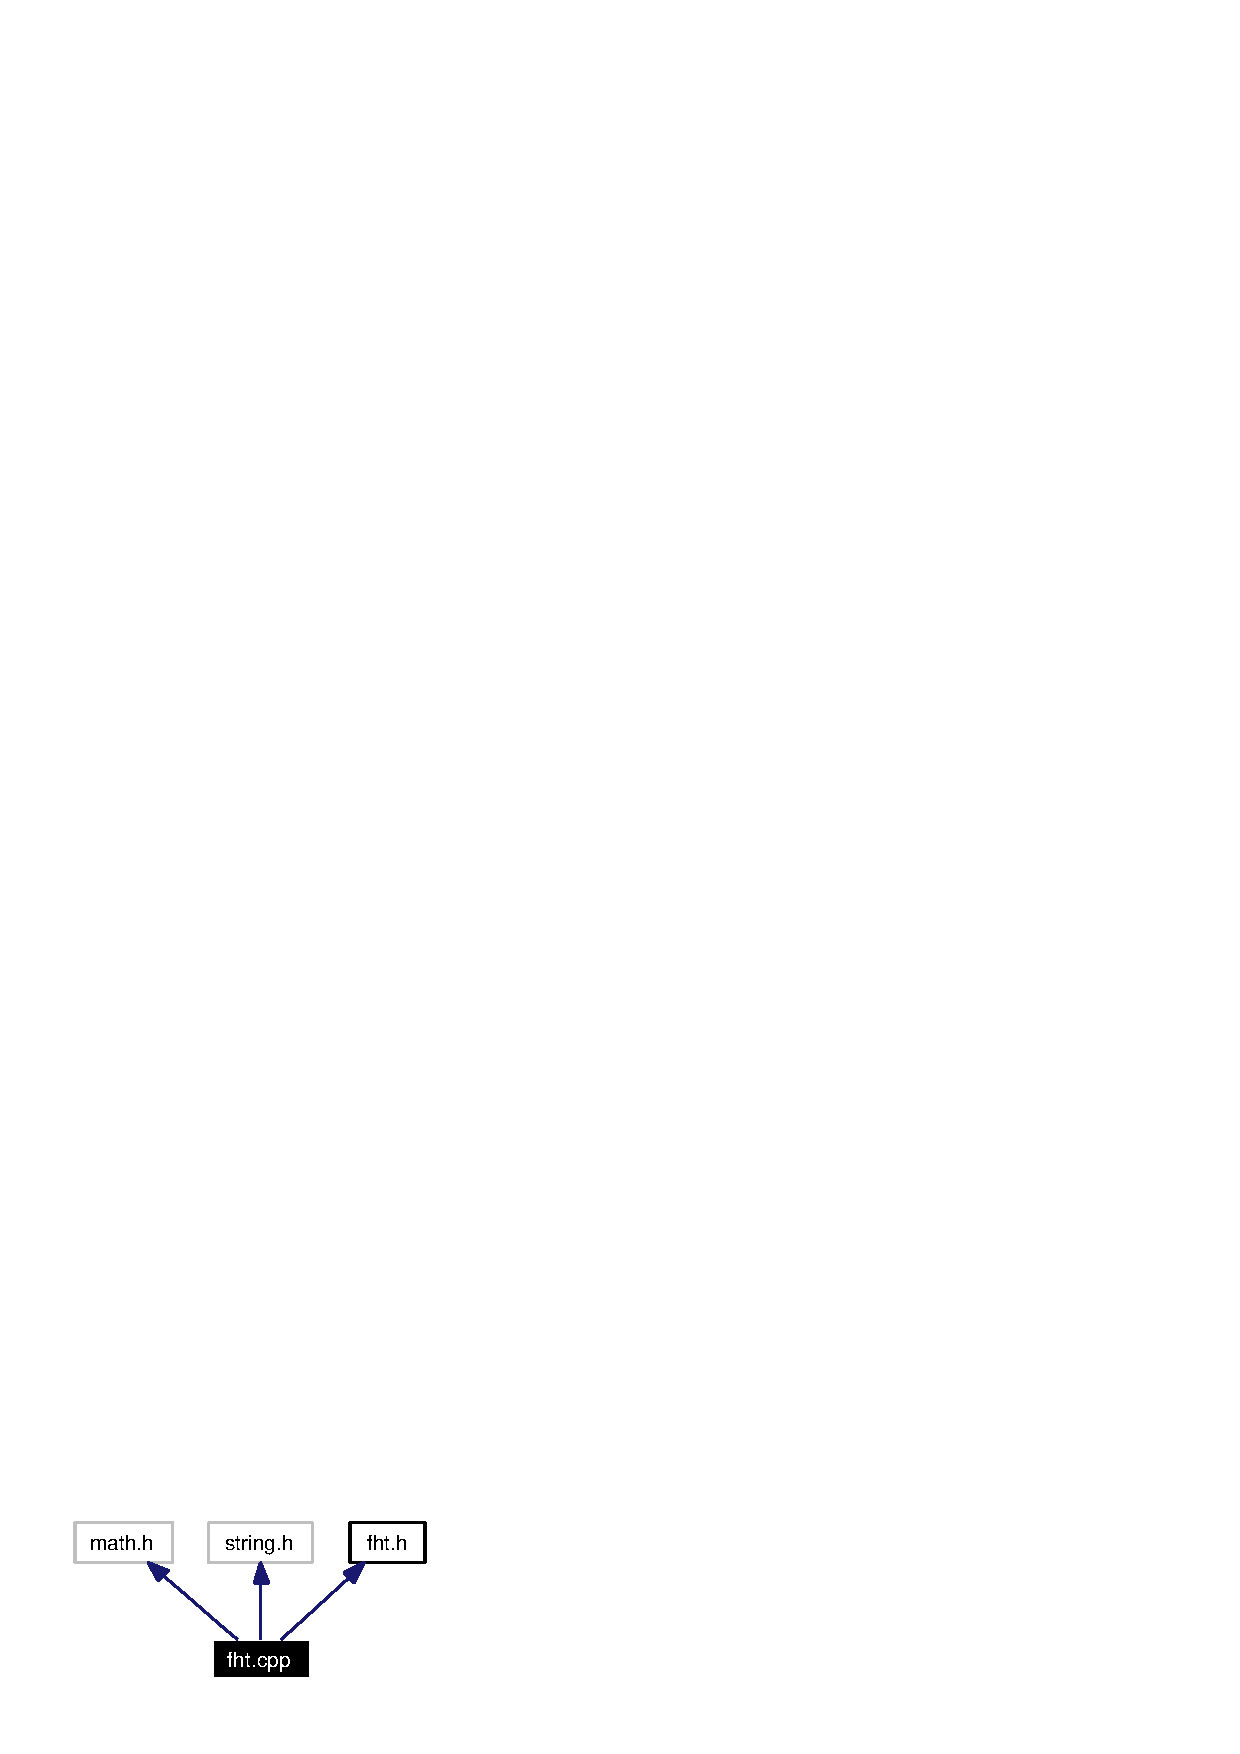
\includegraphics[width=102pt]{fht_8cpp__incl}
\end{center}
\end{figure}
\subsection*{Functions}
\begin{CompactItemize}
\item 
float {\bf sind} (float d)
\end{CompactItemize}


\subsection{Function Documentation}
\index{fht.cpp@{fht.cpp}!sind@{sind}}
\index{sind@{sind}!fht.cpp@{fht.cpp}}
\subsubsection{\setlength{\rightskip}{0pt plus 5cm}float sind (float {\em d})\hspace{0.3cm}{\tt  [inline, static]}}\label{fht_8cpp_a0}




Definition at line 96 of file fht.cpp.

Referenced by FHT::pattern().



\footnotesize\begin{verbatim}96 { return sin(d * M_PI / 180); }
\end{verbatim}\normalsize 
